
% Basic global and layout and formatting information

\documentclass{beamer}
\mode<presentation>
{ \usetheme{simple} }

\pagenumbering{arabic}
\renewcommand{\baselinestretch}{1.8}

% use \rmspace to remove excess vertical space

\newcommand{\rmspace}{\vspace*{-0.25\baselineskip}}

% \usepackage{epsfig} % does not work with pdflatex as of 2011.06
\usepackage{graphicx}
\usepackage{subfigure}
\usepackage{amsmath}

% remove subfigure labeling
\renewcommand{\thesubfigure}{}

\setcounter{figure}{1}



% Set title, author, and talk information [for slide footers] and {title slide}

\title [MR Artifacts] { Common Artifacts in MRI }

\author [Vinai R.] { Vinai Roopchansingh }

\date [2015.06.19] {June 19, 2015}

\institute [FMRIF/NIMH/NIH/DHHS] {Functional MRI Facility, National Institute of Mental Health, National Institutes of Health, Bethesda, MD, USA }

% \email { roopchansinghv@nih.gov }



% have this if you'd like a recurring outline
\AtBeginSection[]  % "Beamer, do the following at the start of every section"
{
   \begin{frame}<beamer> 
   \frametitle{Outline} % make a frame titled "Outline"
   \vspace{-9mm}
   \tableofcontents[currentsection]  % show TOC and highlight current section
   \end{frame}
}



\begin{document}



\begin{frame}

   \titlepage

   \begin{center}

      \vspace {-3mm}

      % \includegraphics[width=75mm]{Pictures/non-EPSs/allLogos.png}

   \end{center}

\end{frame}



\begin{frame}

\frametitle{Outline}

   \vspace {-9mm}

   \tableofcontents

\end{frame}



\section {Hardware artifacts, i.e. B$_0$, B$_1$, etc.}


\begin{frame}

   \frametitle {Hardware imperfections}

   \pause

      \vspace {-36mm}

      \begin{itemize}

         \item <2-> Distortions usually come from B$_0$ or gradient issues.

         \vspace {3mm}

         \item <3-> Image shading/intensity problems usually come from B$_1$ issues.

      \end{itemize}

   \pause

\end{frame}


\begin{frame}

\frametitle{Distortion issues}

   \pause

   \Large

   \vspace{-25mm}

   Larmor equation $\Rightarrow$

   \centering

   \vspace{10mm}

   \LARGE

   \pause $ \omega_0 = \gamma B_0 $

\end{frame}


\begin{frame}

\frametitle{Geometric distortion - Extreme example}

   \pause

   \vspace{-3.0mm}

   \centering

      \includegraphics<2>[width=115mm]{Pictures/non-EPSs/WigArtifactClipPresent.png}

      \includegraphics<3>[width=115mm]{Pictures/non-EPSs/WigArtifactClipAbsent.png}

\end{frame}


\begin{frame}

\frametitle{More common, less extreme, distortion examples}

   \pause

   \vspace{1.0mm}

   \centering

      \includegraphics<2>[width=90mm]{Pictures/non-EPSs/HumanBrainProfileB0.png}

      \includegraphics<3>[width=65mm]{Pictures/non-EPSs/B0_correction_epi2_uncorrected.png}

      \includegraphics<4>[width=65mm]{Pictures/non-EPSs/B0_correction_epi2_corrected.png}

      \includegraphics<5>[width=65mm]{Pictures/non-EPSs/B0_correction_epi_uncorrected.png}

      \includegraphics<6>[width=65mm]{Pictures/non-EPSs/B0_correction_epi_corrected.png}

      \includegraphics<7>[width=65mm]{Pictures/non-EPSs/B0_correction_epi_anatomical_reference.png}

\end{frame}


\begin {frame}

\frametitle {Even more subtle distortion issues}

   \pause

   \vspace{1.0mm}

   \centering

      \includegraphics<2>[width=90mm]{Pictures/non-EPSs/MRI+Gradient.png}

      \includegraphics<3>[width=90mm]{Pictures/non-EPSs/MRI+GradientFieldIdeal.png}

      \includegraphics<4>[width=90mm]{Pictures/non-EPSs/MRI+GradientFieldReal.png}

      \pause

      \includegraphics<5>[width=65mm]{Pictures/non-EPSs/GradientDistortionEPIUncorrected.png}

      \includegraphics<6>[width=65mm]{Pictures/non-EPSs/GradientDistortionEPICorrected.png}

      \includegraphics<7>[width=65mm]{Pictures/non-EPSs/GradientDistortionNoiseScanUncorrected.png}

      \includegraphics<8>[width=65mm]{Pictures/non-EPSs/GradientDistortionNoiseScanCorrected.png}

\end {frame}


\begin {frame}

\frametitle {Very exotic, very troublesome, distortion issue}

   \centering

   \pause

   \includegraphics<2>[width=55mm]{Pictures/non-EPSs/1st_b0_volume.png}
    
   \includegraphics<3>[width=55mm]{Pictures/non-EPSs/2nd_b0_volume.png}

   \includegraphics<4>[width=55mm]{Pictures/non-EPSs/slice14_DW.png}
    
   \includegraphics<5>[width=55mm]{Pictures/non-EPSs/slice15_DW.png}
 
   \tiny Data provided by J. Sarlls

\end {frame}


\begin {frame}

\frametitle {Issues with image intensity, shading, noise}

   \pause

   \Large

   \vspace{-25mm}

   Problems with image intensity variation, noise, etc

   \pause

   $\Rightarrow$ problems along the RF chain

   \pause

   $\Rightarrow$ limitations imposed by physics (geometry, sensitivity).

   \Large

   \vspace{5mm}

   e.g. RF Coils, RF amplifiers, etc.

\end {frame}


\begin {frame}

\frametitle {Failing hardware - single-channel coil}

   \pause

   \vspace{1.0mm}

   \centering

      \includegraphics<2>[width=65mm]{Pictures/non-EPSs/GradientDistortionNoiseScanUncorrected.png}

      \includegraphics<3>[width=65mm]{Pictures/non-EPSs/GradientDistortionEPIUncorrected.png}

\end {frame}


\begin {frame}

\frametitle {Failing hardware - multi-channel array coils}

   % \pause

   \vspace{1.0mm}

   \centering

      \includegraphics<1>[width=65mm]{Pictures/non-EPSs/MultichannelElementGood.png}

      \includegraphics<2>[width=65mm]{Pictures/non-EPSs/MultichannelElementBad.png}

\end {frame}


\begin {frame}

\frametitle {Coil Sensitivity}

    \pause

    \vspace{1.0mm}

    \centering

        \includegraphics<2>[width=65mm]{Pictures/non-EPSs/CoilSensitivity_Profile.png}

        \includegraphics<3>[width=65mm]{Pictures/non-EPSs/CoilSensitivity_002.png}

        \includegraphics<4>[width=65mm]{Pictures/non-EPSs/CoilSensitivity_008.png}

        \includegraphics<5>[width=65mm]{Pictures/non-EPSs/CoilSensitivity_016.png}

        \includegraphics<6>[width=65mm]{Pictures/non-EPSs/CoilSensitivity_025.png}

        \includegraphics<7>[width=65mm]{Pictures/non-EPSs/CoilSensitivity_032.png}

        \includegraphics<8>[width=65mm]{Pictures/non-EPSs/CoilSensitivity_Combined.png}

    \pause

        \includegraphics<10>[width=65mm]{Pictures/non-EPSs/CoilSensitivity_Human.png}

\end {frame}



\begin {frame}

\frametitle {Dielectric Effects / a.k.a. B$_1$ Inhomogeneities}

    \pause

    \vspace{1.0mm}

    \centering

        \includegraphics<2>[width=65mm]{Pictures/non-EPSs/B1EffectAnat.png}

        \includegraphics<3>[width=65mm]{Pictures/non-EPSs/B1EffectEPI.png}

\end {frame}



\section {Reconstruction artifacts}



\begin {frame}

\frametitle {Accelerated Reconstruction artifacts}

    \pause

    \vspace{1.0mm}

    \centering

        \includegraphics<2>[width=65mm]{Pictures/non-EPSs/accelerationFactor1.png}

        \includegraphics<3>[width=65mm]{Pictures/non-EPSs/accelerationFactor2.png}

        \includegraphics<4>[width=65mm]{Pictures/non-EPSs/accelerationFactor3.png}

        \includegraphics<5>[width=65mm]{Pictures/non-EPSs/accelerationFactor4.png}

\end {frame}



\begin {frame}

\frametitle {Error combining data}

    \pause

    \vspace{1.0mm}

    \centering

        \includegraphics<2>[width=90mm]{Pictures/non-EPSs/MultiChannelDataCombineWrong.png}

        \includegraphics<3>[width=90mm]{Pictures/non-EPSs/MultiChannelDataCombineCorrect.png}

\end {frame}



\section {Patient/sample artifacts}



\begin {frame}

\frametitle {Patient/sample artifacts}

    \pause

    \Large

    \vspace{-9.0mm}

    Probably hardest class of artifacts to deal with.

    \begin {itemize}

    \item<3-> Ethical responsibility toward your patients, volunteers, and
              animals.

    \item<4-> Experimental validity - not supposed to change the state of
              the thing you are measuring.

    \end {itemize}

\end {frame}



\begin {frame}

\frametitle {B$_0$ uniformity}

    \pause

    \Large

    \vspace{-12.0mm}

    Basic premise of MRI - {\em VERY} uniform magnetic field, distorted in
    a controlled fashion to provide spatial information.

    \vspace{3.0mm}

    \pause

    $\Rightarrow$ Have to revise this assumption when imaging.

\end {frame}



\begin {frame}

\frametitle {B$_0$ uniformity in the human brain}

    \pause

    \centering

        \includegraphics<2>[width=90mm]{Pictures/non-EPSs/HumanBrainProfileMag.png}

        \includegraphics<3>[width=90mm]{Pictures/non-EPSs/HumanBrainProfileB0.png}

        \includegraphics<4>[width=65mm]{Pictures/non-EPSs/B0_correction_epi2_uncorrected.png}

        \includegraphics<5>[width=65mm]{Pictures/non-EPSs/B0_correction_epi2_corrected.png}

        \includegraphics<6>[width=65mm]{Pictures/non-EPSs/B0ThroughSliceSignalLoss.png}

\end {frame}



\begin {frame}

\frametitle {Different tissue types, namely fat}

    \pause

    \centering

        \includegraphics<2>[width=65mm]{Pictures/non-EPSs/B0_correction_epi_corrected.png}

        \includegraphics<3>[width=65mm]{Pictures/non-EPSs/fatline_slc39_vol13.jpg}

\end {frame}



\begin {frame}

\frametitle {Physiology}

    \pause

    \centering

    \vspace{-1mm}

        \includegraphics<2>[width=110mm]{Pictures/non-EPSs/vanGelderenRespirationPhase.png}

    van Gelderen: Magnetic Resonance In Medicine (57:2), 362-368, Feb 2007.

\end {frame}



\begin {frame}

\frametitle {Motion}

    \pause

    \centering

    \vspace{-1mm}

        \includegraphics<2>[width=110mm]{Pictures/non-EPSs/Motion_001.png}

        \includegraphics<3>[width=110mm]{Pictures/non-EPSs/Motion_002.png}

        \includegraphics<4>[width=110mm]{Pictures/non-EPSs/Motion_003.png}

        \includegraphics<6>[width=100mm]{Pictures/non-EPSs/motionYes.png}

        \includegraphics<7>[width=100mm]{Pictures/non-EPSs/motionNo.png}

\end {frame}



\section {Misc. / grab-bag}



\begin {frame}

\frametitle {EPI Nyquist Ghosting}

    \pause

    \centering

        \includegraphics<2>[width=110mm]{Pictures/non-EPSs/n2NyquistGhostNormal.png}

        \includegraphics<3>[width=110mm]{Pictures/non-EPSs/n2NyquistGhostArtifact.png}

\end {frame}



\begin {frame}

\frametitle {Saturation effects}

    \pause

    \centering

        \includegraphics<2>[width=110mm]{Pictures/non-EPSs/Saturation_001.png}

        \includegraphics<3>[width=110mm]{Pictures/non-EPSs/Saturation_002.png}

        \includegraphics<4>[width=110mm]{Pictures/non-EPSs/Saturation_003.png}

        \includegraphics<5>[width=110mm]{Pictures/non-EPSs/Saturation_004.png}

\end {frame}



\begin {frame}

\frametitle {Pop-quiz}

    \pause

    \vspace{-35mm}

    \begin {itemize}

    \item<2> How to differentiate fat shift artifact from Nyquist ghost shift ?

    \end {itemize}

\end {frame}



\begin {frame}

\frametitle {Pop-quiz}

    \vspace{-2mm}

    \centering

        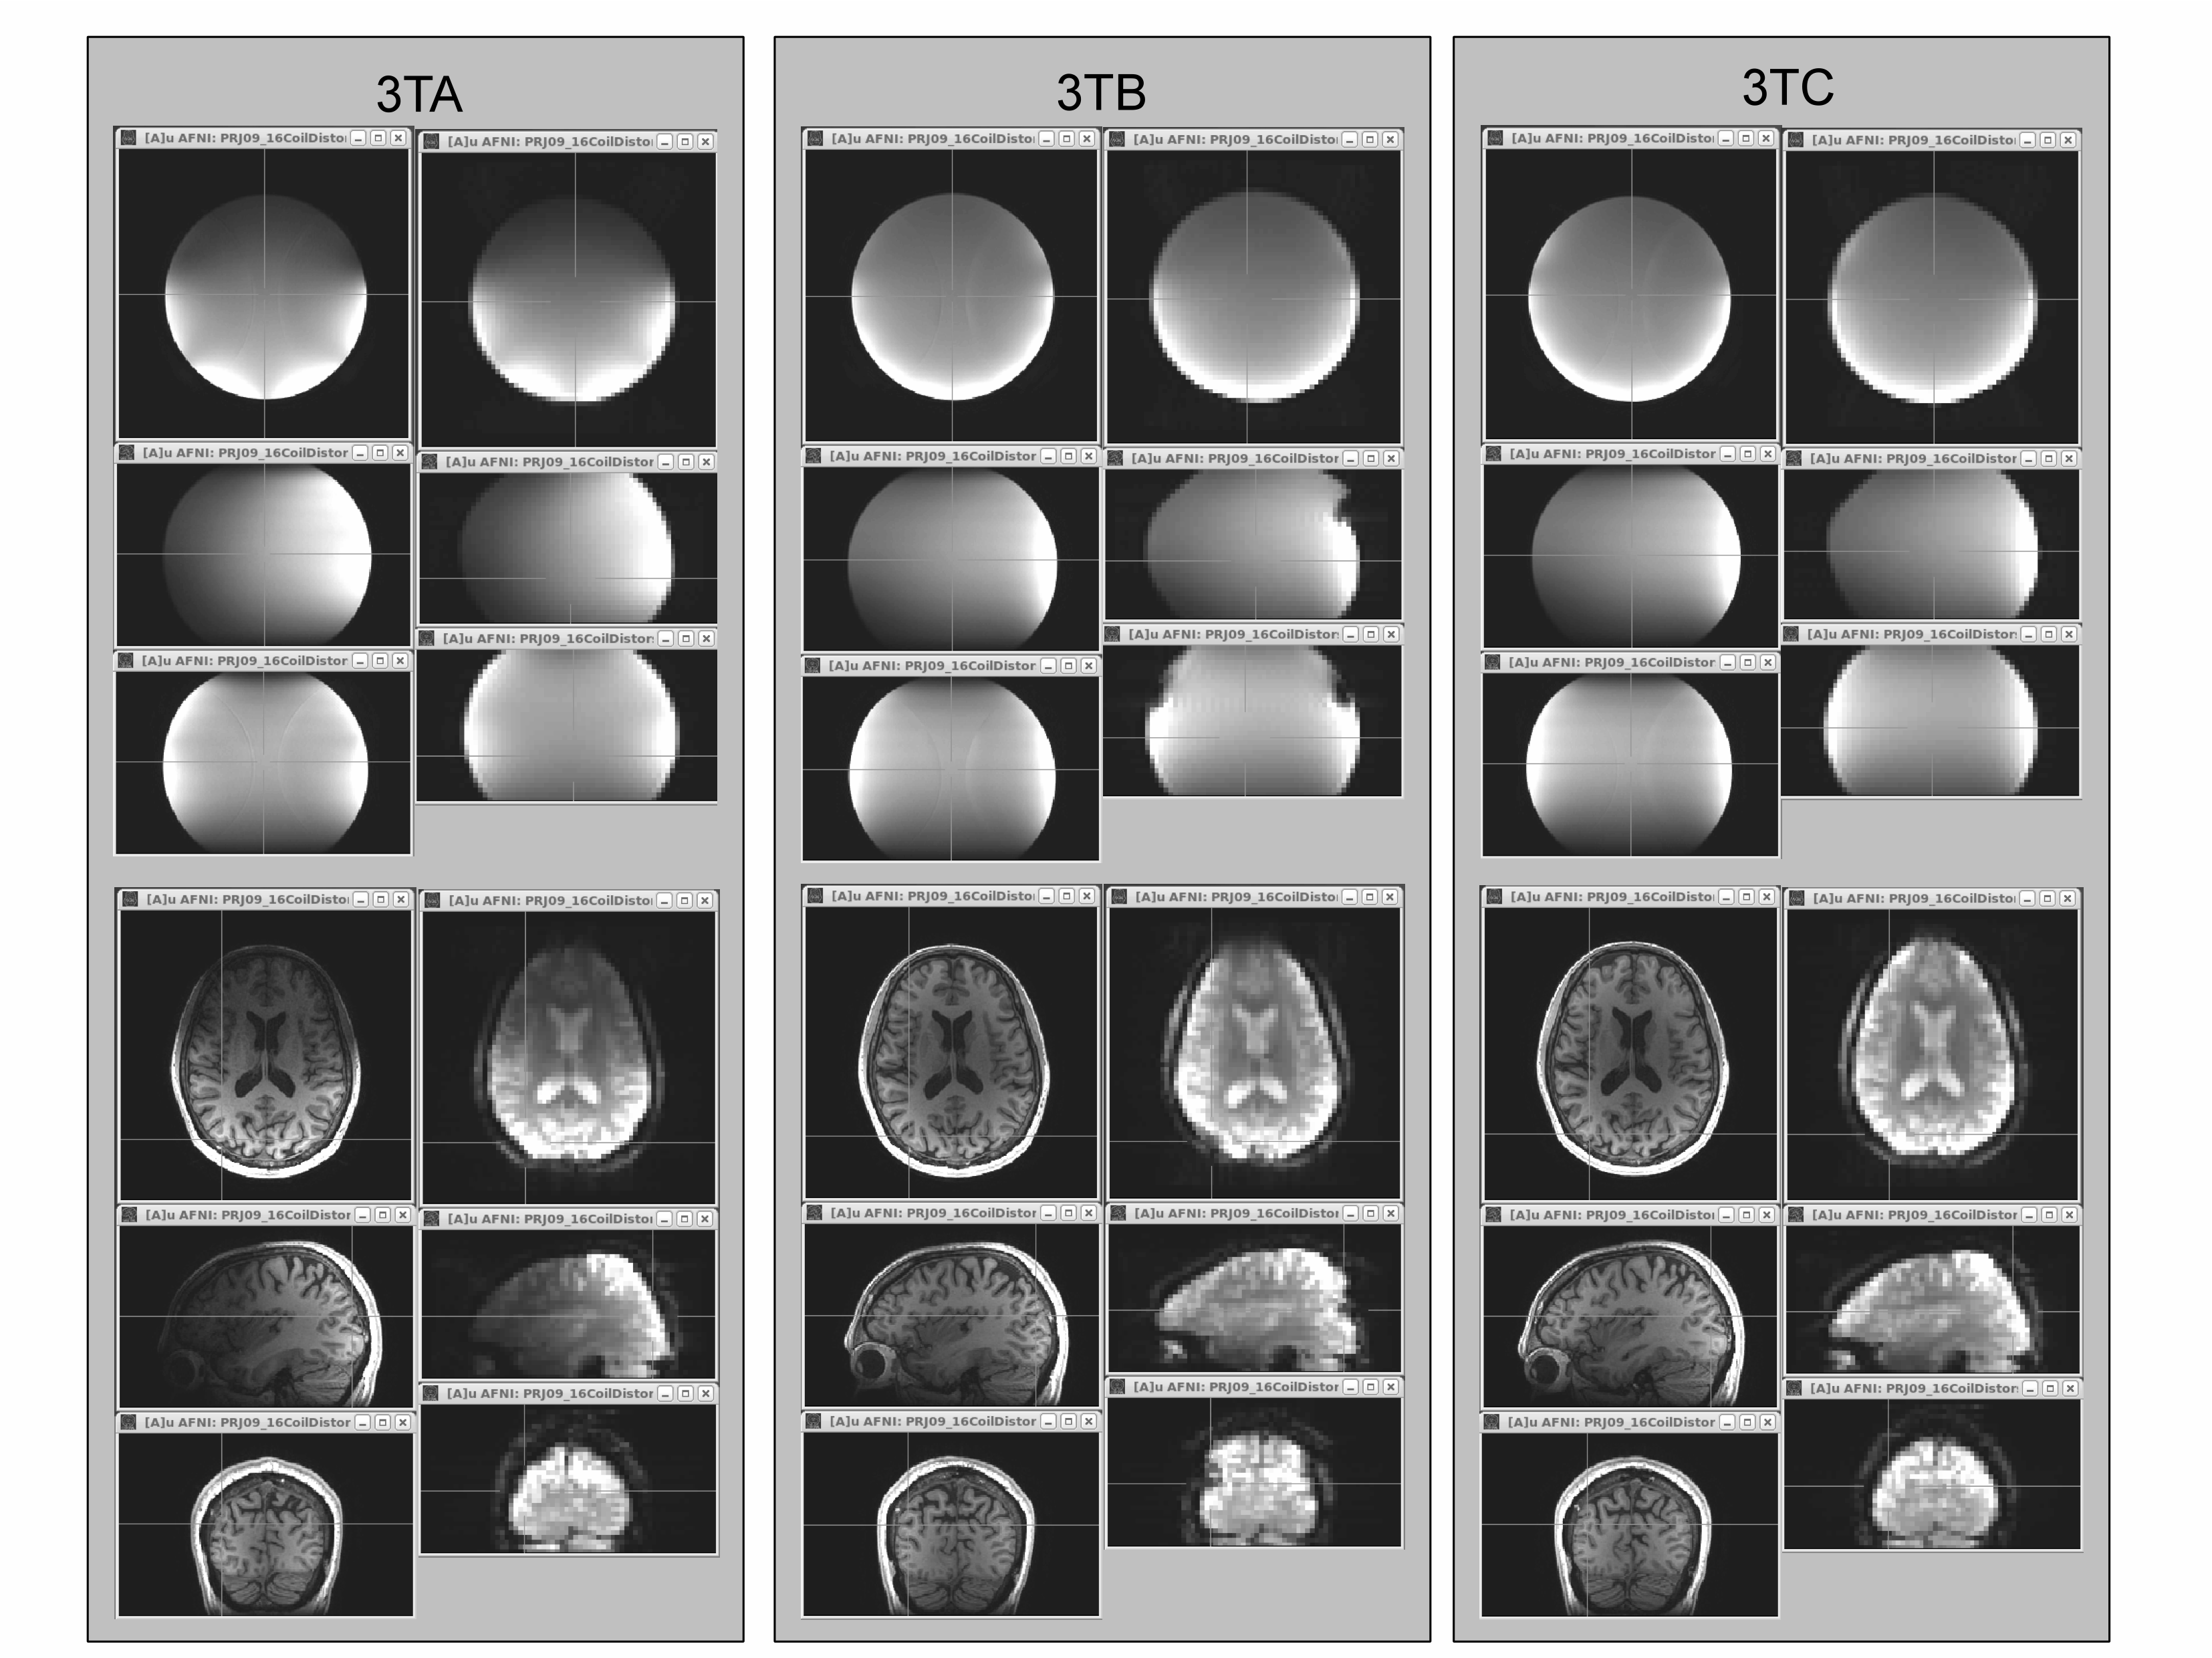
\includegraphics[width=99mm]{Pictures/non-EPSs/NovaCoilComparison.png}

\end {frame}



\begin {frame}

\frametitle {Acknowledgments}

    \vspace{-25mm}

    \begin {itemize}

        \item J. Sarlls (NMRF-NINDS)

        \item R. M. Birn (MCW/FIM-NIMH/UW)

        \item S. Wei and S. Kippenhan (SIN-NIMH)

        \item J. Gonzalez-Castillo (FIM-NIMH)

        \item D. Handwerker (FIM-NIMH)

    \end {itemize}

\end {frame}



\end{document}

